%%%%%%%%%%%%%%%%%%%%%%%%%%%%%%%%%%%%%%%%%%%%%%%%%%%%%%%%%%%%%%%%%%%%%%%%%%%%%%%%
%2345678901234567890123456789012345678901234567890123456789012345678901234567890
%        1         2         3         4         5         6         7         8

\documentclass[letterpaper, 10 pt, conference]{ieeeconf}  % Comment this line out if you need a4paper

%\documentclass[a4paper, 10pt, conference]{ieeeconf}      % Use this line for a4 paper

\IEEEoverridecommandlockouts                              % This command is only needed if 
                                                          % you want to use the \thanks command

\overrideIEEEmargins                                      % Needed to meet printer requirements.

% TODO They are called left and right lane boundaries

%In case you encounter the following error:
%Error 1010 The PDF file may be corrupt (unable to open PDF file) OR
%Error 1000 An error occurred while parsing a contents stream. Unable to analyze the PDF file.
%This is a known problem with pdfLaTeX conversion filter. The file cannot be opened with acrobat reader
%Please use one of the alternatives below to circumvent this error by uncommenting one or the other
%\pdfobjcompresslevel=0
%\pdfminorversion=4

% See the \addtolength command later in the file to balance the column lengths
% on the last page of the document

% The following packages can be found on http:\\www.ctan.org
%\usepackage{graphics} % for pdf, bitmapped graphics files
%\usepackage{epsfig} % for postscript graphics files
%\usepackage{mathptmx} % assumes new font selection scheme installed
%\usepackage{times} % assumes new font selection scheme installed
\usepackage{amsmath} % assumes amsmath package installed
\usepackage{amssymb}  % assumes amsmath package installed
\usepackage[utf8x]{inputenc}
\usepackage{graphicx}

% for code listings
\usepackage{color}
\usepackage[usenames,dvipsnames]{xcolor}
\usepackage{listings}

% General style options, mostly controlling line numbers
\lstset{
	frame            = lines,
	showstringspaces = false,
	numbers          = left,          % Line numbers left
	numberstyle      = \color{black}, % Line numbers are black, not deepblue
	breaklines       = true,          % Wrap overly-long lines
}
\definecolor{deepblue}{rgb}{0,0,0.5}
\definecolor{deepred}{rgb}{0.6,0,0}
\definecolor{deepgreen}{rgb}{0,0.5,0}

% Python style from https://tex.stackexchange.com/questions/83882/how-to-highlight-python-syntax-in-latex-listings-lstinputlistings-command/83883#83883

% Python style for highlighting
\lstdefinestyle{Python}{
	language         = Python,
	basicstyle       = \ttfamily\footnotesize,     % Font style (fixed width) and size
	otherkeywords    = {self,True,False},     % Add keywords you want to take keywordstyle here
	keywordstyle     = \bfseries\color{blue},
	emph             = {__init__,__name__,},  % Custom highlighting, add important things
	emphstyle        = \color{red}\bfseries,       % Custom highlighting style
	stringstyle      = \color{deepgreen}, % Color of "strings"
	commentstyle     = \color{deepred},   % Color of #comments
}



\title{\LARGE \bf
Designing an API for Autonomous Vehicle Steering Controllers
}


\author{Emiko Soroka${}^1$ and Sanjay Lall${}^2$
%\thanks{*This work was not supported by any organization}% <-this % stops a space
%\thanks{}%
%\thanks}%
}

\makeatletter
\newcommand{\makefootnote}[2]{{
  \def\@thefnmark{#1}
  \@footnotetext{#2}
}}
\makeatother

\begin{document}




\newcommand{\ms}{\text{m}/\text{s}}
\newcommand{\kmh}{\text{km}/\text{h}}
\newcommand{\vdes}{v_{\text{des}}}

\maketitle
\thispagestyle{empty}
\pagestyle{empty}


\makefootnote{1}{S. Lall is Professor of Electrical
  Engineering at Stanford University, Stanford, CA 94305, USA.
  \texttt{lall@stanford.edu}\medskip}

\makefootnote{2}{E. Soroka is a PhD student in Aeronautics and Astronautics at Stanford University, Stanford, CA 94305, USA. \texttt{esoroka@stanford.edu}\medskip}
%%%%%%%%%%%%%%%%%%%%%%%%%%%%%%%%%%%%%%%%%%%%%%%%%%%%%%%%%%%%%%%%%%%%%%%%%%%%%%%%
\begin{abstract}

Software reusability is critical to the rapid development and certification of autonomous vehicles (AVs). However, little attention has been given to designing AV controllers for increased software reusability. In this paper we approach the design task from a reusability perspective to specify an API between higher-level AV action planning and lower-level trajectory optimization. Clearly defining this interface confines hardware dependencies to the lower-level trajectory planning module, improving software reusability. We implement a nonlinear MPC controller in simulation to demonstrate the feasibility of this API in common traffic scenarios. % TODO fix
\end{abstract}


%%%%%%%%%%%%%%%%%%%%%%%%%%%%%%%%%%%%%%%%%%%%%%%%%%%%%%%%%%%%%%%%%%%%%%%%%%%%%%%%
\section{INTRODUCTION}

Advanced driver assistance systems (ADAS) and autonomous vehicles are a rapidly growing segment of the automotive industry. However, the rise of automotive software presents new challenges in software reusability.
% TODO In the introduction we might mention ASIL V, a functional safety thing: automotive safety integrity level. THe other thing is ISO 26262. Both of these are standards that enforce regulations about how the software that controls functional parts of the car must be written. The point is automotive companies have to certify the software against ASIL and ISO 26262 and if you can have a software system which can be certified and reused, that's "a huge win". So we should expand a little more on this point by mentioning these standards. There's a company called Apex.Ai that takes things like ROS and make a version which is ASIL and ISO 26262 certified.
Developing an autonomy stack for a single vehicle is only the first step in bringing AVs to market. After developing a prototype AV, manufacturers need to adapt their stack to vehicles with different capabilities. Software reuse is a key component of this process: if the stack can be certified once under standards such as ASIL and ISO 26262, then deployed to other platforms, AV manufacturers can rapidly enter all segments of the vehicle market.

Autonomous route planning, object recognition, and other high-level decision-making processes are hardware-agnostic. However, steering and acceleration control is tightly coupled to specific hardware. To optimize fuel efficiency, for example, a gasoline-powered vehicle must be driven differently than an electric-gas hybrid or fully electric vehicle with regenerative braking. In emergency situations, knowledge of tire-road interactions, vehicle inertia, center of gravity, and engine performance is critical to averting an accident \cite{beal}. Thus, lower level control algorithms are much less portable between different vehicles.

We approach AV steering and acceleration control from a software reusability perspective. We propose that an optimizing controller, requiring only information about its environment and desired behavior, removes hardware dependencies in higher-level modules and improves AV software reusability. Moreover, this approach allows the desired driving behavior to be changed without re-tuning the controller. The proposed interface decreases software development and certification requirements.


\section{THE AV STEERING AND ACCELERATION CONTROL PROBLEM}
\subsection{Configurability}
Major concerns with steering and acceleration control for autonomous vehicles include fuel efficiency, passenger comfort, and safety. However, different applications of autonomy put different weight on these objectives. An autonomous truck delivering cargo prioritizes fuel efficiency. An autonomous taxi must avoid maneuvers that would cause discomfort or alarm to customers. Many ADAS-equipped vehicles in today's market offer the option of switching between different driving modes, for example `sport' and `eco-friendly' modes, which change the vehicle's performance. This suggests that fully autonomous consumer vehicles would be expected to offer the same type of configurable experience.


\subsection{Division at Waypoints}

To reduce hardware dependencies, one could seek to simplify the low-level controller. Suppose our high-level software plans driving maneuvers (such as turning, stopping, or maintaining a safe distance from another vehicle) and decomposes these maneuvers into a trajectory of closely spaced waypoints specifying the vehicle's state over time. The low level controller tracks this trajectory. Unfortunately, without hardware knowledge informing the trajectory generation, the vehicle follows a sub-optimal path, limiting its ability to handle dynamic emergency situations.

\subsection{Division at Maneuvers} Alternatively, suppose we divide the software where driving maneuvers are specified. The low-level controller receives data about these maneuvers, such as the road boundaries and specific, desired states (such as stopping at a stop sign or maintaining a safe distance behind another car). The controller then computes a trajectory using hardware-specific information. For example, a hybrid with regenerative braking can recover electric energy, while a vehicle without this capability may spend more time coasting to a stop and less time actively braking. A vehicle on a wet road can steer more conservatively. The trajectory optimization is coupled to the hardware, providing a performance benefit that must be weighed against the development cost of the optimizing controller.

\subsection{The Design Task}
In this paper we divide hardware-dependent and -independent software at the level of driving maneuvers: the low-level controller receives a driveable corridor, desired speed, and specific objectives. The controller then computes a trajectory using hardware-specific knowledge. We propose an interface between low level and high level software capable of representing arbitrary driving maneuvers and present an example controller.

\section{PRIOR WORK}

\subsection{Classical Control for Trajectory Tracking}
PID controllers can be applied to steering and acceleration control; however, tuning the PID gains remains challenging. Mohajer et al. define a multi-objective problem to evaluate a trajectory for efficiency and passenger comfort, then apply a genetic algorithm to optimize their controller's PID gains offline \cite{pid}. This significantly reduces path tracking error and undesirable high-frequency control inputs over their baseline of hand-tuned PID gains. However, information about the vehicle's hardware is required to complete the PID tuning. The authors use 28 numerical parameters describing the vehicle's geometry, inertia matrices, and shock absorber performance to simulate the PID controller during the optimization process. This suggests in a practical application, the tuning procedure would need to be rerun for a variety of different configurations.


Classical control can be applied to complex vehicle models. Chebly et al. develop a multi-body model of the vehicle, using 21 bodies connected by joints to represent the chassis, suspension, steering, and wheels \cite{CHEBLY201712526}. Their work uses 12 parameters including vehicle mass, inertia, and cornering stiffnesses of tires. The high fidelity of this vehicle model enables the steering and acceleration controller to perform well in highly nonlinear situations \cite{CHEBLY201712526}. The authors also discuss the controller's robustness to errors caused by variations in the vehicle's mass or tire stiffness, verifying the controller can continue to track the reference trajectory with a $\pm30\%$ error in these parameters.

\subsection{MPC Trajectory Tracking}
Farag et al. apply MPC trajectory tracking to achieve high performance on tracks featuring tight curves and hairpin turns \cite{farag}. Notably, this performance is achieved with only two parameters: the distances $l_f$ and $l_r$ from the vehicle's center of mass to its front and rear wheels, respectively. The authors use a simple kinematic bicycle model for the vehicle, noting that this increases the algorithm's portability to different vehicles.

These simpler models appear in many MPC algorithms. Daoud et al. propose  a dual-objective nonlinear MPC formulation for trajectory tracking, allowing an electric vehicle to switch between driving modes \cite{pathfollowingMPC}. They use the kinematic bicycle model with an additional simplification: the center of gravity (CG) is assumed to be at the center of the wheelbase. Only one parameter is needed: the wheelbase length $l$. The front and rear axles are a distance $l/2$ away from the CG. An additional parameter describes electric motor efficiency. 

Finally, Beal et al. develop an MPC tracking controller for stabilizing a vehicle during extreme maneuvers \cite{beal}. Their approach uses a more detailed model, including tire behavior, to account for the complex dynamics of these situations.

\subsection{Trajectory Optimization}

There are fewer trajectory planning controllers, likely due to the increased difficulty of design. Li et al. apply an inner model control framework to split the task into 2 parts: first, given a safe corridor, a trajectory and optimal control input is computed. Then an inner model controller driven by this signal is used to account for disturbances in the vehicle \cite{pathtracking}. The authors selecte a bicycle model with three parameters: $l_r$, $l_f$, and vehicle mass. They also use a linear approximation to model tire forces with two parameters for front and rear tire stiffness.

More recently, NMPC has been applied to directly compute the vehicle's state and control signals \cite{nmpc_micheli}. Micheli et al. use penalties and hard constraints to represent road boundaries, static obstacles, and moving obstacles in the nonlinear optimization problem.
Though NMPC is computationally difficult, zero-order optimization approaches are also possible: Arrigoni et al. use genetic algorithms to solve the difficult nonlinear optimization problem in real time \cite{arrigoni2021mpc}. NMPC trajectory planning has also been demonstrated on real AV hardware \cite{nmpc_platform}.

\section{AN API FOR AV TRAJECTORY PLANNERS}

We propose the following division (Fig. \ref{fig:block}), focusing on the Trajectory Planning module. We define an API for the module's inputs and outputs and provide an example controller that implements our interface.

\begin{figure}[h]
	\centering
	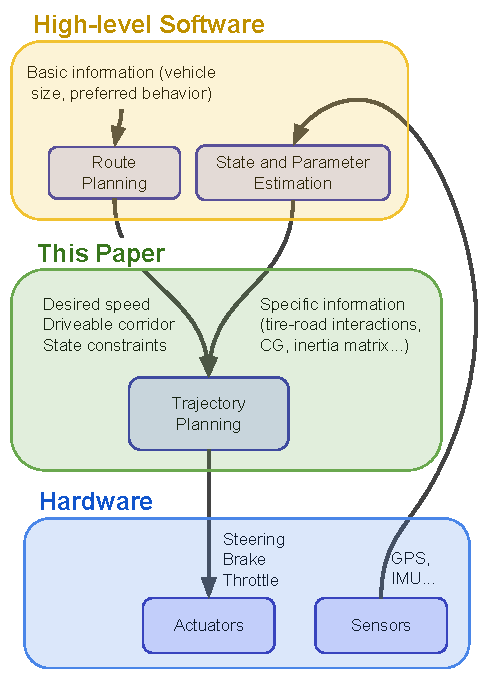
\includegraphics[width=0.7\linewidth]{figures/block_diagram.pdf}
	\caption{Block diagram showing how this paper fits into a larger autonomy stack.}
	\label{fig:block}
\end{figure}

The proposed controller is initialized with vehicle-specific information, some of which may be estimated or changed over time (for example, tire-road friction parameters). In addition it may query three functions provided by higher-level software, described below.

\subsection{Desired Speed}
The desired speed is an estimate of the vehicle's speed provided by higher-level software: for example, the speed of other traffic. The controller is not required to remain at this speed if a minor deviation yields improvement in other objectives.

The desired speed is a function of position and timestep: the vehicle can accelerate according to some profile. Providing both position and time enables the function to represent moving obstacles.
The function accepts a point $(x, y)$ in the driveable corridor and a timestep index $k \in 1,\dots,N$, then returns the desired speed at step $k$: $v_{des,k}$ (a floating-point value).
%
$$\texttt{desired\_speed($x,\ y,\ k$)}\rightarrow v_{des,k}$$
This can be used to construct a list of desired speeds for $N$ timesteps: $v_{des} = [v_{des,1},\dots,v_{des,N}]$.

% TODO Spell it out explicitly and explicitly link the math to the code.
% TODO Overall, explicitly link math to code and functions.


\subsection{Driveable Corridor} \label{sub:corridor}
% TODO Should we discuss that the road is a union of discs? We have a representation that doesn't depend on time.

The driveable corridor function takes the vehicle's current position $(x,y)$ and an offset $s$, returning a new center point $(x_c, y_c)$ and angle $\psi_c$ a distance $s$ away from $(x,y)$. Additionally, it returns the distances to the left and right boundaries $d_l$ and $d_r$ (measured perpendicular to the center line) at $(x_c, y_c)$ (Fig. \ref{fig:corridor}).
%
$$\texttt{driveable\_corridor($x,\ y,\ s$)} \rightarrow (x_c, y_c, \psi_c, d_l, d_r)$$
%
The center point is not necessarily the geometric center of the corridor. Providing two distances allows turnouts and wide shoulders to be represented (Fig. \ref{fig:corridor_with_shoulder}). 
Additionally, the driveable corridor is not necessarily the entire road. If an obstacle encroaches on the road, the corridor will be reduced.
Finally, the corridor representation fails to account for obstacles with free space on both sides. This will be addressed in Section \ref{sub:constraints}.


\begin{figure}[h]
	\centering
	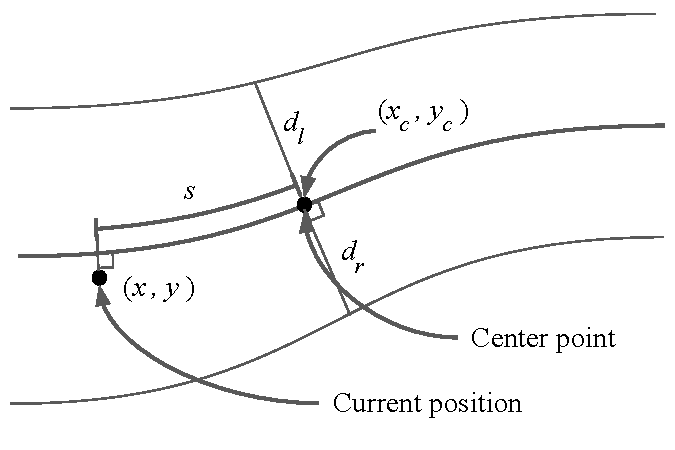
\includegraphics[width=0.9\linewidth]{figures/corridor.pdf}
	\caption{The driveable corridor function accepts the current position $(x,y)$ and offset $s$, then returns a new position $(x_c, y_c)$ and distances $d_l$ and $d_r$ a distance $s$ away from the current position.}
	\label{fig:corridor}
\end{figure}

\begin{figure}[h]
	\centering
	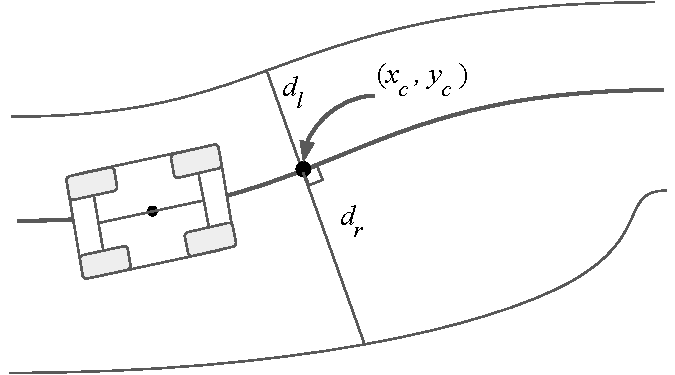
\includegraphics[width=0.9\linewidth]{figures/corridor_with_turnout.pdf}
	\caption{This road has a wide shoulder. Using a left and right distance allows the centerline to represent the ``center" a reasonable human driver would follow, which may not be the geometric center.}
	\label{fig:corridor_with_shoulder}
\end{figure}


% TODO Describe how this function is used.
% TODO Describe how that information changes. What changes this information? The vehicle moving, the repeated computation, moving obstacles, etc.
% TODO How are obstacles dealt with?

\subsection{State Constraints}\label{sub:constraints}
State constraints allow high-level software to ensure a safety or legal requirement is met. For example, a constraint could ensure the vehicle has 0 velocity at an $x-y$ position corresponding to a stop sign. A time-dependent constraint could limit position to ensure a minimum following distance behind another
vehicle. Finally, a constraint could keep the vehicle away from an obstruction in the driveable corridor. This accounts for the situation mentioned in Section (\ref{sub:corridor}).

\begin{figure}[h]
	\centering
	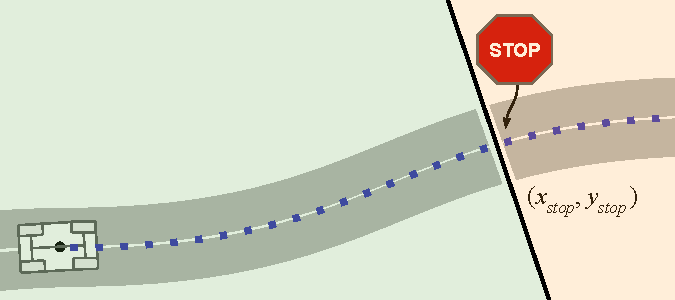
\includegraphics[width=0.9\linewidth]{figures/stop.pdf}
	\caption{When stopping, the vehicle must stay behind the line. Its position is constrained using a linear inequality to restrict it to the green region.} 
	\label{fig:stopsign}
\end{figure}

\begin{figure}[h]
	\centering
	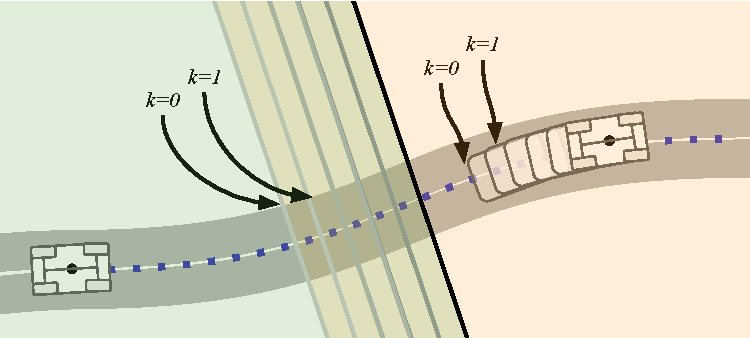
\includegraphics[width=0.9\linewidth]{figures/following.pdf}
	\caption{The ego vehicle is following another car. The linear inequality moves at each timestep $k=1,\dots,N$. to enforce a minimum safe distance.}
	\label{fig:vehicle_in_front}
\end{figure}

\begin{figure}[h]
	\centering
	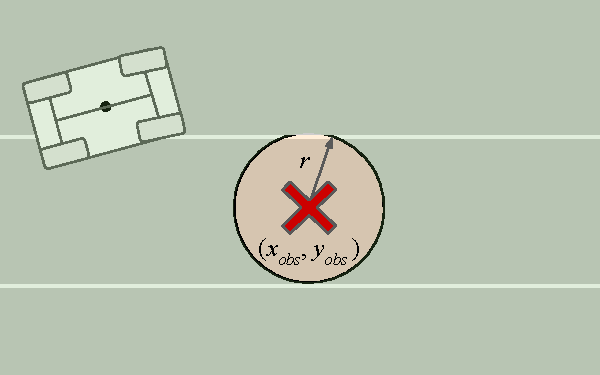
\includegraphics[width=0.9\linewidth]{figures/obstacle_in_road.pdf}
	\caption{An obstacle (X) obstructs one lane, creating a circular keep-out region of radius $r$. The vehicle must stay out of the circle, creating a nonconvex constraint $(x-x_{obs})^2 + (y-y_{obs})^2 \geq r$}
	\label{fig:obstacle}
\end{figure}


To accommodate these and other situations, a constraint generator function takes an $x-y$ position, a speed $v$ (which may be the desired or estimated speed), and a timestep $k=1,\dots,N$. It returns a function $g$ representing a vector of inequality constraints on $x_k, y_k, v_k$: the vehicle's position and speed at timestep $k$. These constraints may be nonlinear and nonconvex (Fig. \ref{fig:obstacle}).
%
$$\texttt{constraint\_generator($z_k,\ k$) ->} g(\cdot, \cdot, \cdot)$$

The constraints are satisfied at step $k$ if $g(z_k) \leq 0$ (where $z_k = \begin{bmatrix}
x_k& y_k& \psi_k& v_k
\end{bmatrix}$ is the state vector).



 \section{IMPLEMENTATION}
 
We implemented a nonlinear MPC (NMPC) controller using this interface. To model the vehicle, we used a kinematic bicycle model \eqref{eq:kinematic}, also used in \cite{farag} and shown in Fig. \ref{fig:kinematic}. There are two system parameters: $l_f$, the distance from the center of mass (CoM) to the front axle, and $l_r$, the distance from the CoM to the rear axle. We used $l_r = 2.10\ \text{m}$ and $l_f = 2.67\ \text{m}$ for all simulations: the same values as \cite{farag}.
 
 \begin{figure}[htbp]
 	\centering
 	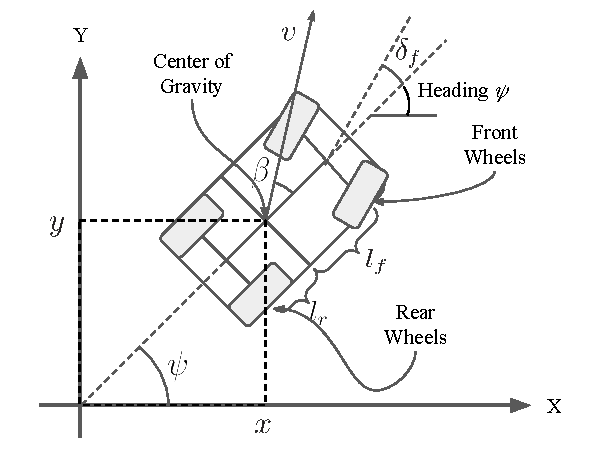
\includegraphics[width=0.8\linewidth]{figures/kinematic_diagram.pdf}
 	\caption{Kinematic bicycle model.}
 	\label{fig:kinematic}
 \end{figure}
 

 \begin{equation}
 z = \begin{bmatrix}
 x\\y\\v\\\psi
 \end{bmatrix},\quad \begin{bmatrix}
 \dot x\\\dot y\\\dot v\\\dot\psi
 \end{bmatrix} = \begin{bmatrix}
 v\cos(\psi + \beta)\\
 v\sin(\psi + \beta)\\
 a\\
 \frac{v}{l_r}\sin(\beta)
 \end{bmatrix}
 \label{eq:kinematic}
 \end{equation}
 
 \begin{equation}
 \beta = \tan^{-1}\Big( \frac{l_r}{l_f + l_r}\tan(\delta_f) \Big)
 \label{eq:beta}
 \end{equation}
 
 The control signals are $a$, the longitudinal acceleration of the car, and $\delta_f$, the steering angle of its front wheels. The control vector is $u = [a\ \delta_f]\ \in \mathbb{R}^2$.
 
 We consider an NMPC problem with lookahead steps $k=1,\dots,N$ with $N=30$ steps spaced a distance $\Delta_t = 0.075\ \text{s}$ apart. The nonlinearity is confined to the dynamics model \eqref{eq:kinematic} and constraints (Fig. \ref{fig:obstacle}). The cost function is quadratic.
 
In our implementation, we used the driveable corridor function to generate a list of linear inequalities representing the road as shown in Fig. \ref{fig:roadpolygons}. Each right and left boundary constrains the vehicle's $x-y$ position at one step: for $N$ lookahead steps, $2N$ lines are generated. Arbitrarily tight curvatures can be represented by decreasing the time between each step (Fig. \ref{fig:roadpolygons}).

 \begin{figure}[h]
 	\centering
 	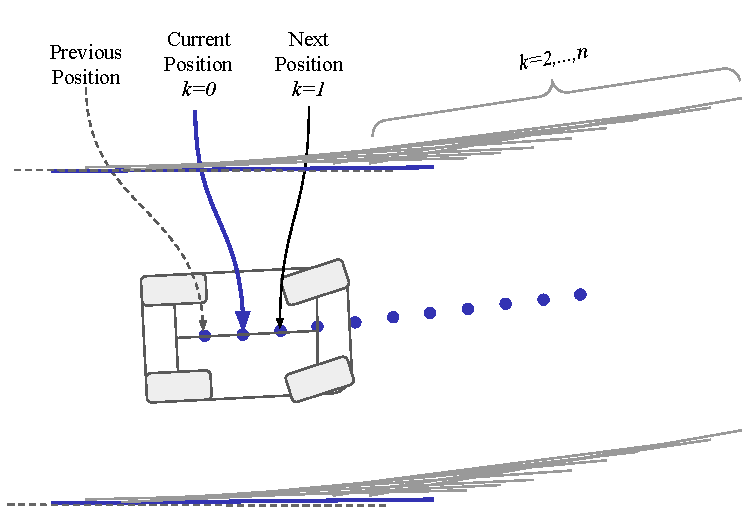
\includegraphics[width=0.9\linewidth]{figures/road_final_bounds.pdf}
 	\caption{A short sample of overlapping lines to define the road corridor. 2 lines are used to constrain the vehicle's position at eack step $k$.}
 	\label{fig:roadpolygons}
 \end{figure}
 
 \subsection{Cost function}
Our multi-objective cost function penalizes sharp accelerations which degrade passenger comfort and deviations from the desired speed and center of the driveable corridor. We use 2 terms to control this accuracy:
 
 \begin{equation}
 J_{\text{accuracy}} = \sum_{k=1}^N\big\| \begin{bmatrix}
 x_k\\y_k\\\psi_k
 \end{bmatrix} - \begin{bmatrix}
 x_{\text{center},k}\\y_{\text{center},k}\\\psi_{\text{center},k}
 \end{bmatrix} \big\|_2^2
 \label{eq:costcenter}
 \end{equation}
  \begin{equation}
 J_{\text{speed}} = \sum_{k=1}^N (v_k - v_{\text{des},k})^2
 \label{eq:speed}
 \end{equation}
 %
 where $(x_{\text{center},k},\ y_{\text{center},k},\ \psi_{\text{center},k}$ is returned by \texttt{driveable\_corridor} and $v_{\text{des},k}$ is returned by \texttt{desired\_speed}. These functions are provided by higher-level software (Fig. \ref{fig:block}).
 
 % TODO Rerpesente x, y, psi as lists from 1,k,...N and mention them in the code to relate the functions to the MPC problem defined in equations 9,...14
 
 % TODO Using f(...) twice in equation 9 and in the defiition of the constraint generator
 % TODO The constraint generator should return a list of scalar constraints in case we have a situation with more than one constraint.
 
 Equation \eqref{eq:costcenter} controls path-following accuracy, while \eqref{eq:speed} controls how closely the vehicle stays at the desired speed. Because the desired speed could be small or large, \eqref{eq:costcenter} and \eqref{eq:speed} are separated so they can be weighted differently.
 
 
 Equations \eqref{eq:costjerk} and \eqref{eq:coststeering} penalize undesirable sharp changes in acceleration ($\text{m}/\text{s}^2$) and steering angle (deg).
 
 \begin{equation}
 J_{\text{jerk}} = \sum_{k=2}^N (a_k - a_{k-1})^2
 \label{eq:costjerk}
 \end{equation}
 
 \begin{equation}
 J_{\text{accel}} = \sum_{k=2}^N (\delta_{f,k} - \delta_{f,k-1})^2
 \label{eq:coststeering}
 \end{equation}
 
 By separating these terms, they can be weighted to produce different behaviors \eqref{eq:costfinal}.
 \begin{equation}
 J = a_1 J_{\text{accuracy}} + a_2 J_{\text{speed}} + a_3 J_{\text{jerk}} + a_4 J_{\text{steering}} + a_5J_{\text{accel}}
 \label{eq:costfinal}
 \end{equation}
 
 We use the notation $z$ to denote a list of states $z_1,\dots,z_N$ and controls $u=u_1,\dots,u_N$.
 The final NMPC problem is:
 \begin{align}
 \text{minimize}\quad& J(z, u)
 \\
 \text{subject to} \quad& z_{k} = f(z_{k-1}, u_{k-1}),\ k=1,\dots,N
 \\
 & u_{\min} \leq u \leq u_{\max}
 \\
 & v_{\min} \leq v \leq v_{\max}
 \\
 & \psi_{\min} \leq \psi \leq \psi_{\max}
 \\
 &
 A_k\begin{bmatrix}
 x_k\\y_k\\
 \end{bmatrix} \geq 0,\ k=1,\dots,N
 \\
 &
g(x_k, y_k, \psi_k, v_k) \leq 0,\ k=1,\dots,N
 \end{align}
 where $A_k$ is a matrix of linear inequalities constructed from \texttt{driveable\_corridor} and \texttt{desired\_speed} describing the corridor boundaries at the $k$th step.
 
 
 \subsection{Implementation Details}
The $x-y$ position of the vehicle is constrained by the linear inequalities, so there is no need to impose any other condition on it. The velocity was constrained to $0 \leq v \leq 50\ \ms$.
The control signals were limited to $-5 \leq a \leq 2.5$ and $-\pi/4 \leq \delta_f \leq \pi/4$.
 
 The problem was defined using CasADi in Python and solved with ipopt \cite{Casadi} \cite{ipopt}. Ipopt requires initialization when solving a nonlinear optimization problem: an estimated speed and position must be provided. Using the solution of the $k$th problem as the initial guess for the $k+1$th NMPC problem provided a significant reduction in computation time.
 
 We provide an outline of this implementation:
 \begin{lstlisting}[caption={Nonlinear MPC controller using proposed API.},style=Python]
 class TrajectoryPlanner():
     def run(self, initial_state:np.array,
                   driveable_corridor  :callable,
                   desired_speed       :callable,
                   constraint_generator:callable):
     # See section IV for definitions of these callables
     self.z0 = initial_state
     self.initialize_first_mpc_problem(driveable_corridor, desired_speed, constraint_generator)
 
     while True:
         # Construct the MPC problem
         problem = self.build_mpc_problem(driveable_corridor, desired_speed, constraint_generator)
         # Compute the trajectory z and control u: a list of states and control signals from 1,..N
         z, u    = self.solve_mpc_problem(problem)
         # Move forward one timestep
         self.z0 = self.apply_control(u[0])
         # Initialize next problem with previous result
         self.initialize_nth_mpc_problem(z, u)
 \end{lstlisting}
 
 %
%          # Use the callables to step along the road
% x = [self.z0[0],]; y = [self.z0[1],]
% v = [self.z0[2],]; psi = [self.z0[3],]
% for k in range(1, N):
% x_k, y_k, psi_k = driveable_corridor(x[k-1], y[k-1], T*v[k-1])
% v_k = desired_speed(x_k, y_k, k)
% x.append(x_k);     y.append(y_k)
% psi.append(psi_k); v.append(v_k)
 
 
 \section{Results} % TODO Fix
 We tested the controller on three scenarios. In the double-lane-change simulation, the vehicle is driving at $10\ \ms$ ($36\ \kmh$) and must navigate the ISO double lane-change path. The steering accuracy and the magnitude of the control signals is evaluated.
 
 The stop sign scenario consists of a straight road with a stop sign. The vehicle is driving at $4\ \ms$ ($14.4\ \kmh$), detects the stop sign from 10 m away, and must smoothly come to a stop.
 
Finally, the vehicle following scenario consists of a straight road with another vehicle. The ego vehicle is initially driving at $4\ \ms$ but must slow down to maintain a minimum safe distance behind a slower driver.

 \subsection{Double lane change}
 
In this scenario, we tested a range of weights for the cost function \eqref{eq:costfinal}. Accuracy terms \eqref{eq:costcenter} and \eqref{eq:speed} were grouped. Jerk \eqref{eq:costjerk} and steering change terms \eqref{eq:coststeering} were also grouped.
 
 Initial tuning was performed to keep the grouped terms within an order of magnitude of each other, resulting in a cost function with one adjustable weight $a$:
 $$J = \Big( J_{\text{accuracy}} + 10^3J_{\text{speed}} \Big) + a\Big( 10J_\text{{jerk}} + 10J_\text{{accel}} + J_{\text{steering}}\Big),$$
 A large value of $a$ corresponds to a high weight on comfort (smaller and smoother control signals) while a small value corresponds to a high weight on position and speed accuracy.
 Results are provided for several weights of $a$ to illustrate this tradeoff.
 In practice the weights would be application-dependent or adjusted on the fly as discussed in \cite{nmpc_micheli}.
 
 
 \begin{figure}[h]
 	\centering
 	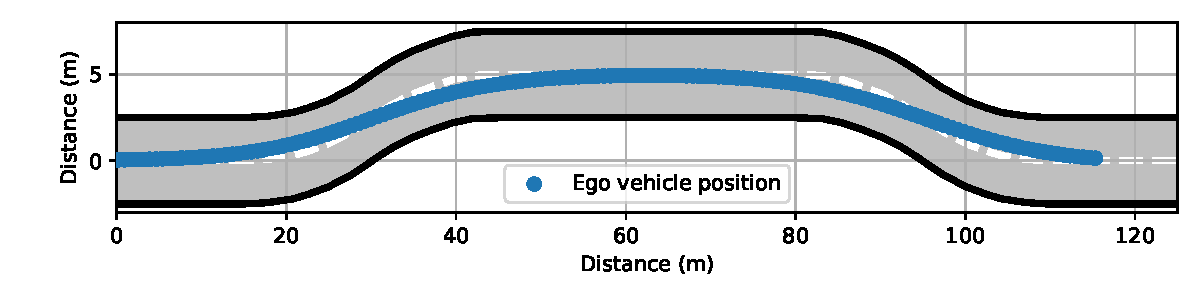
\includegraphics[width=1.0\linewidth]{figures/double_lane_change.pdf}
 	\caption{The double-lane-change scenario. The road width is 5 m and the desired speed is $10\ \ms$. To minimize jerk and sharp changes in steering angle, the vehicle deviates from the road centerline.}
 	\label{fig:trajectory(lanechange)}
 \end{figure}
 
 %\begin{figure}[h]
% 	\centering
% 	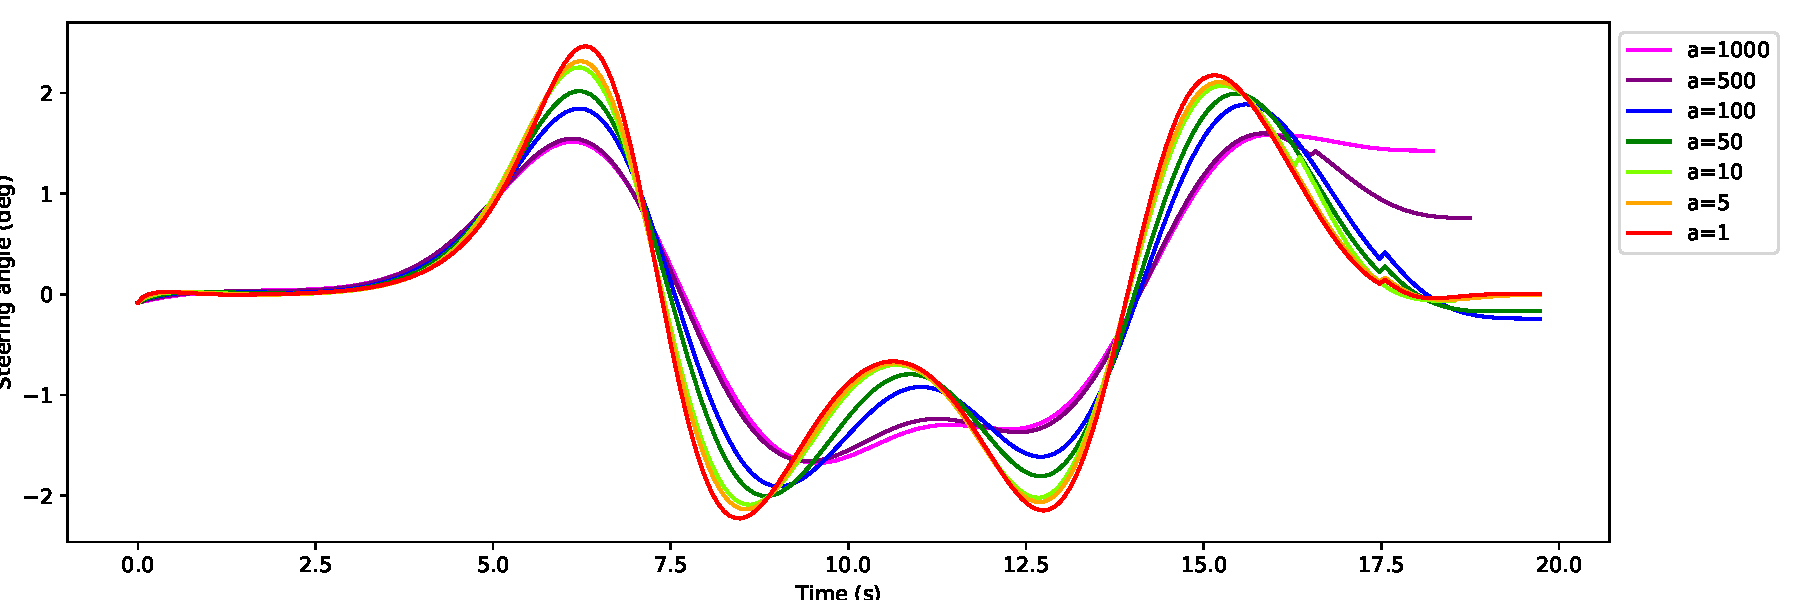
\includegraphics[width=1.0\linewidth]{figures/Steering(lanechange).pdf}
% 	\caption{Steering signal (in degrees) for the double-lane-change scenario.}
% 	\label{fig:steering(lanechange)}
% \end{figure}
 
 \begin{figure}[h]
 	\centering
 	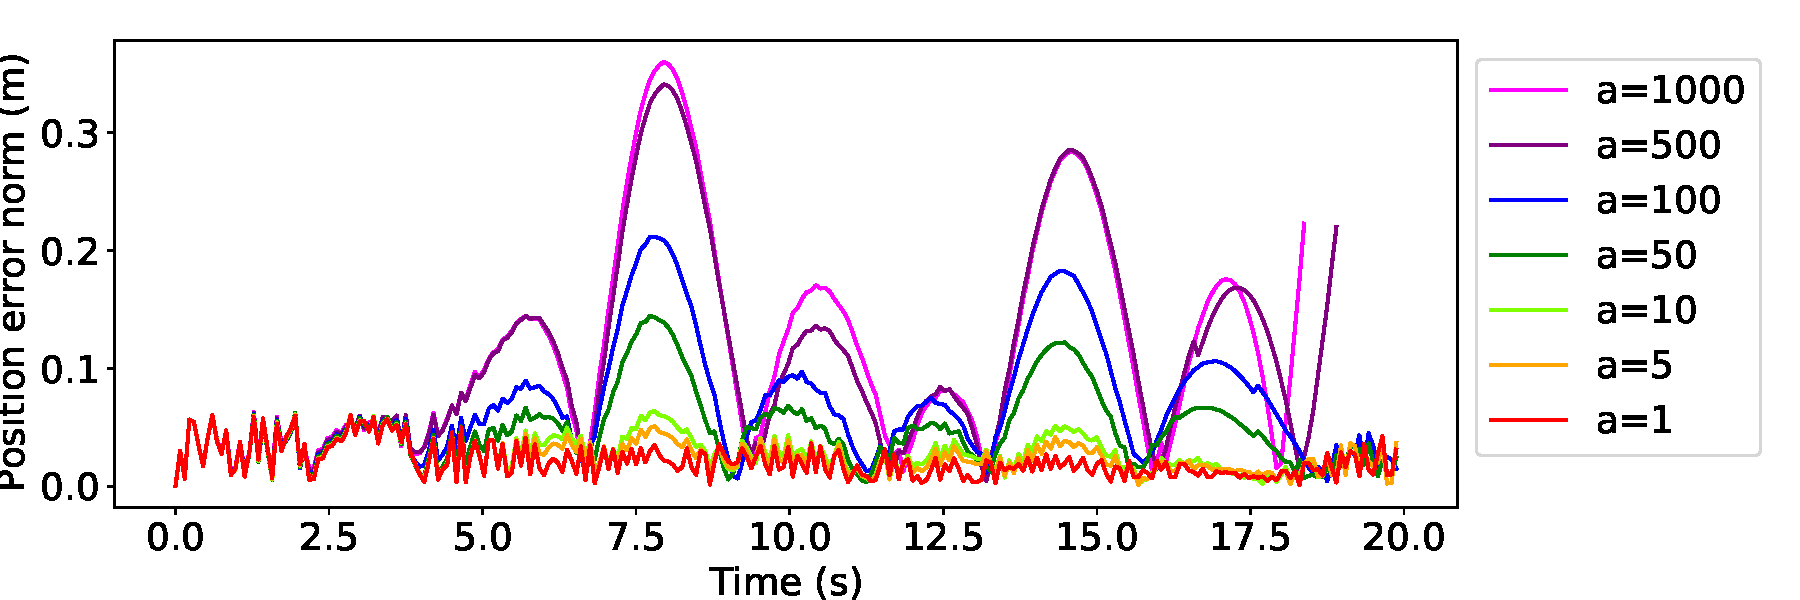
\includegraphics[width=1.0\linewidth]{figures/Position_error(lanechange).pdf}
 	\caption{Position error from the road centerline (meters) in the double-lane-change scenario with different MPC weights.}
 	\label{fig:error(lanechange)}
 \end{figure}
 
 As expected, the position error is low for high accuracy runs and increases for high comfort runs (Fig. \ref{fig:error(lanechange)}).
 % Additionally, the $a=1000$ and $a=500$ runs are very similar in Fig. \ref{fig:steering(lanechange)} and \ref{fig:error(lanechange)}, suggesting larger values of $a$ would not result in meaningfully smaller acceleration/jerk values.
 
 \subsection{Stop sign}
 
 %\begin{figure}[h!]
% 	\centering
% 	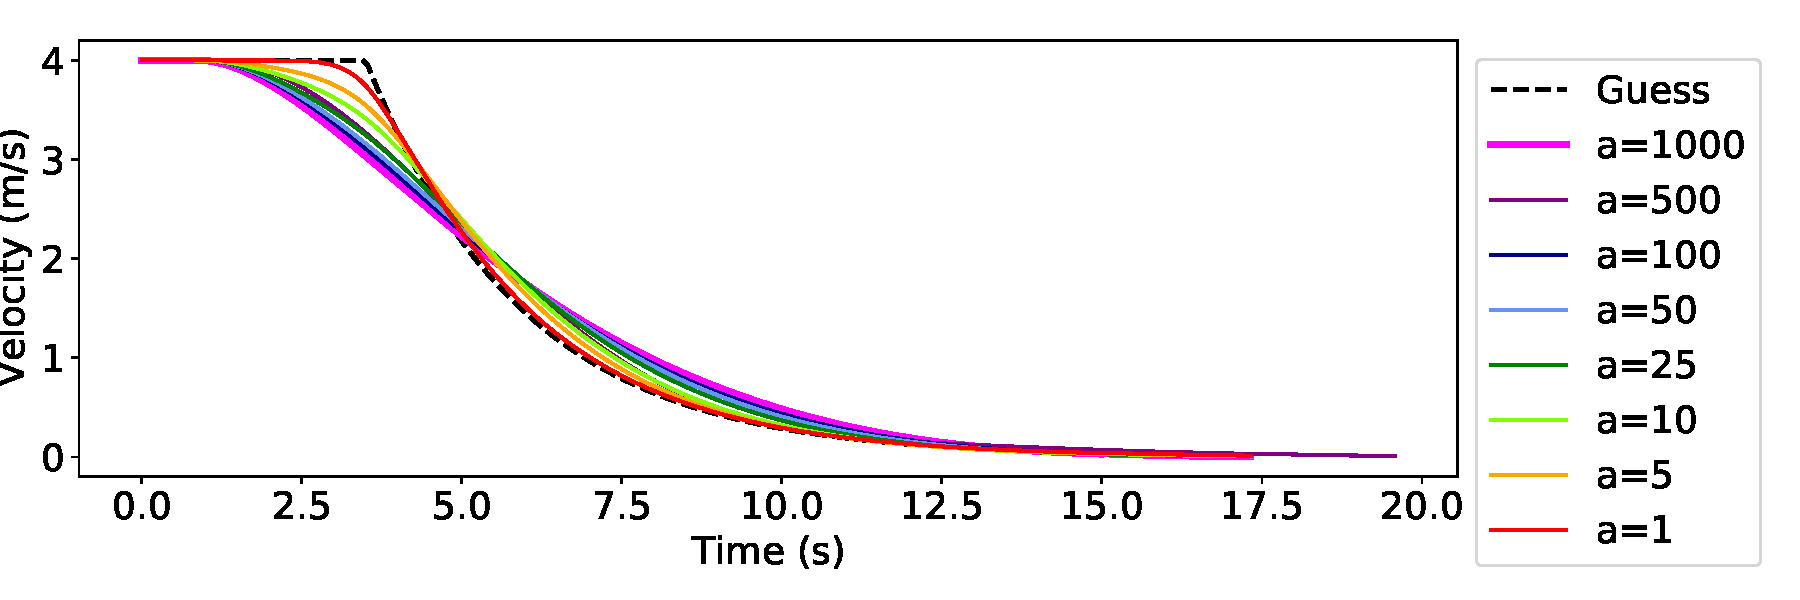
\includegraphics[width=1.0\linewidth]{figures/Velocity_time(stop).pdf}
% 	\\
% 	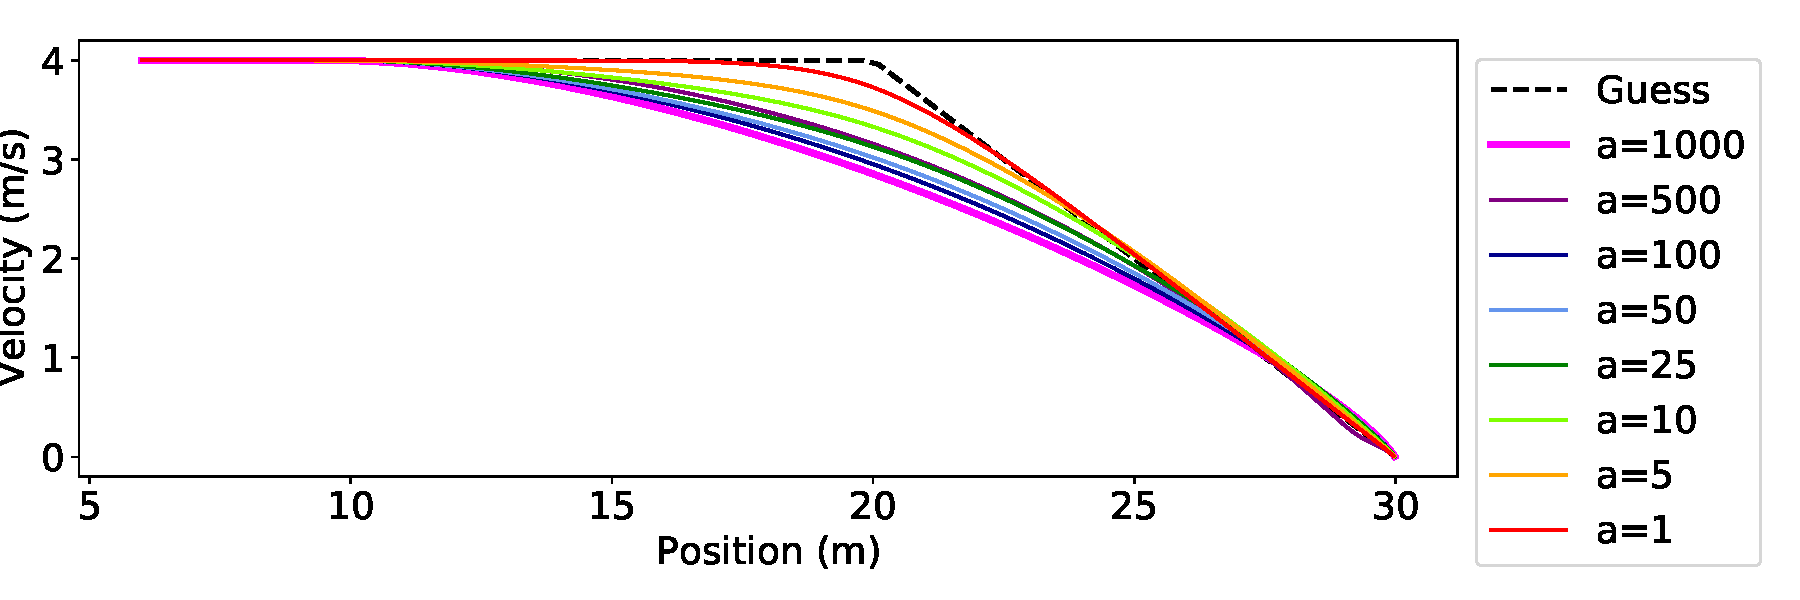
\includegraphics[width=1.0\linewidth]{figures/Velocity_position(stop).pdf}
% 	\caption{Velocity vs time (top) and position(bottom) for the stop sign scenario. The desired or estimated velocity decreases linearly with position.}
% 	\label{fig:velocity(stop)}
% \end{figure}
 
\begin{figure}[h!]
	\centering
	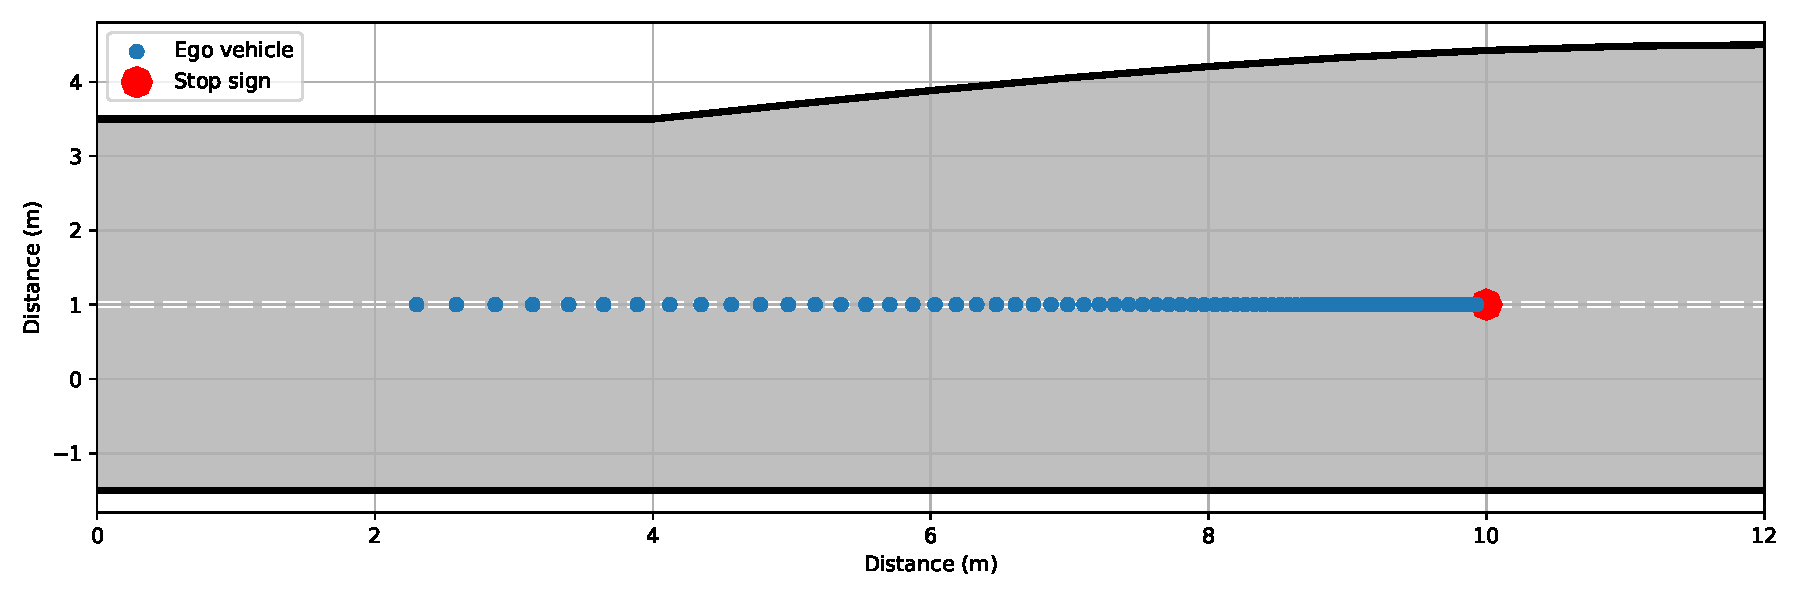
\includegraphics[width=1.0\linewidth]{figures/stop_sign.pdf}
	 	\vspace{-1.5em}
	\caption{Using a hard constraint to enforce 0 velocity at a stop sign.}
		\label{fig:stop_sign}
\end{figure}
 
% \begin{figure}[h!]
% 	\centering
% 	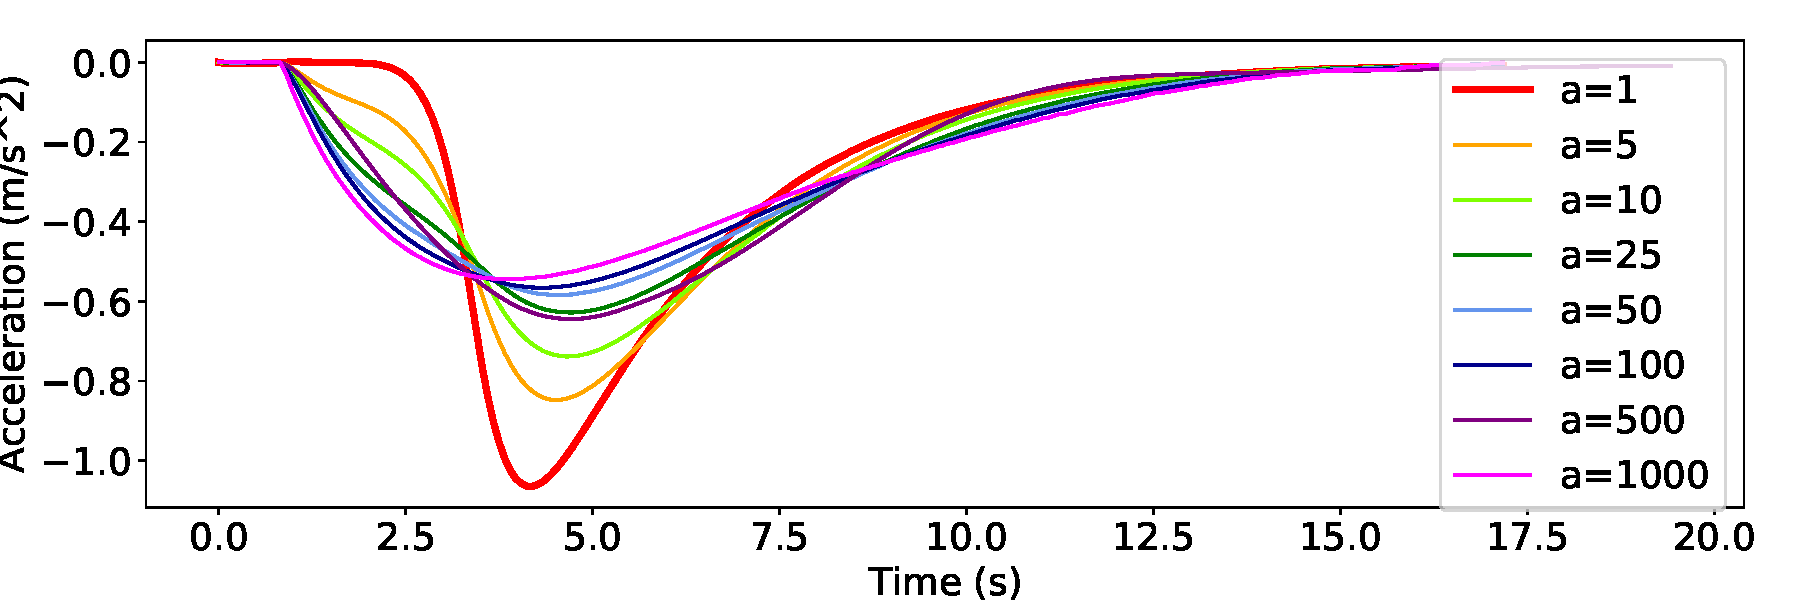
\includegraphics[width=1.0\linewidth]{figures/Acceleration(stop).pdf}
% 	\\
% 	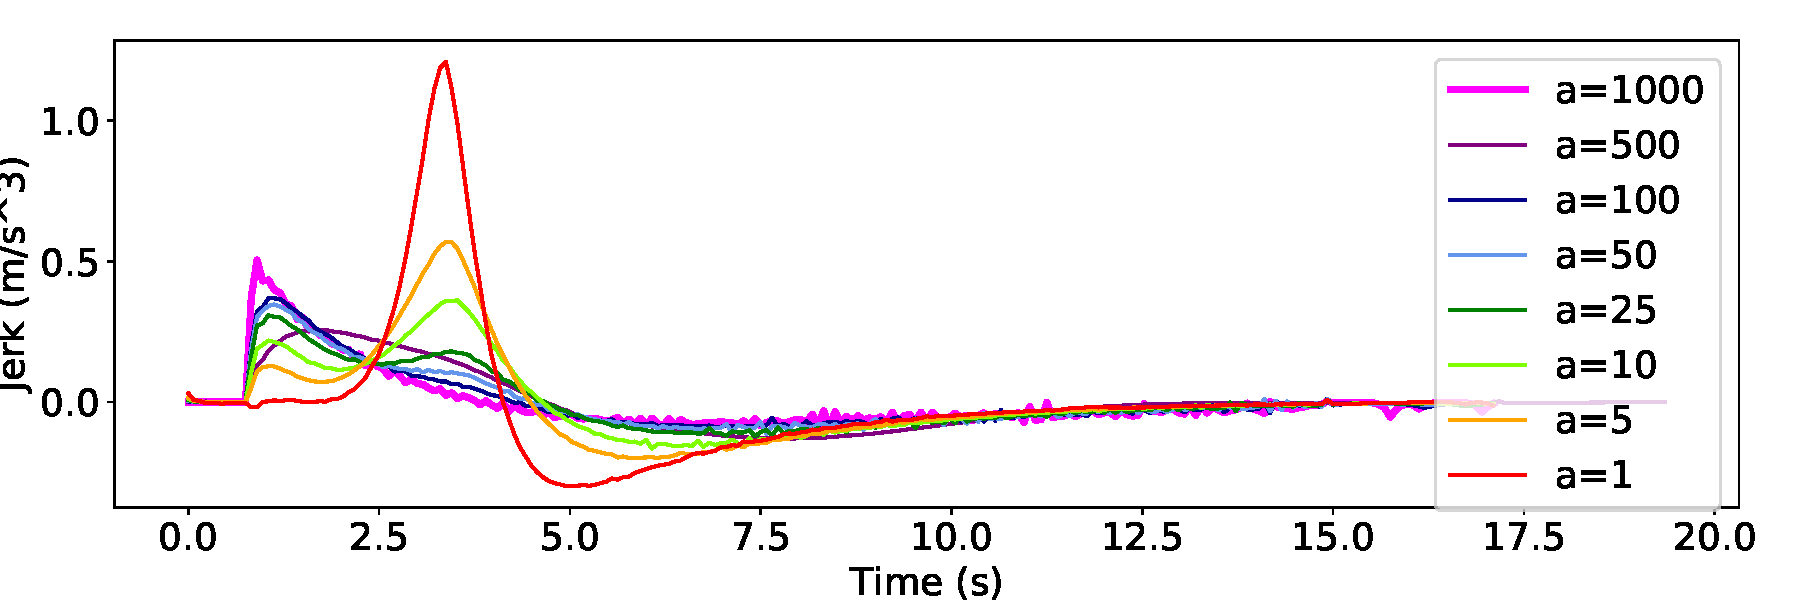
\includegraphics[width=1.0\linewidth]{figures/Jerk(stop).pdf}
% 	\caption{Acceleration signal (top, $\text{m}/\text{s}^2$) and jerk (bottom, $\text{m}/\text{s}^3$) for the stop sign scenario with different MPC weights.}
% 	\label{fig:acceleration_jerk(stop)}
% \end{figure}
% 
 In this test, the road is straight: the car never deviates from the road centerline so there is no position error as defined in Fig. \ref{fig:error(lanechange)}. Similarly, the steering signal remains at 0. The goal is to minimize acceleration and jerk.
 
The desired velocity profile was a rough estimate: the velocity was set at $4\ \ms$ until the stop sign is detected at $10\ \ms$ away; after that it decreases linearly (with distance) to 0. Despite this discontinuity, the NMPC controller produces a smooth velocity profile (Fig. \ref{fig:stop_sign_velocity}).
 
 \begin{figure}[h!]
 	\centering
 	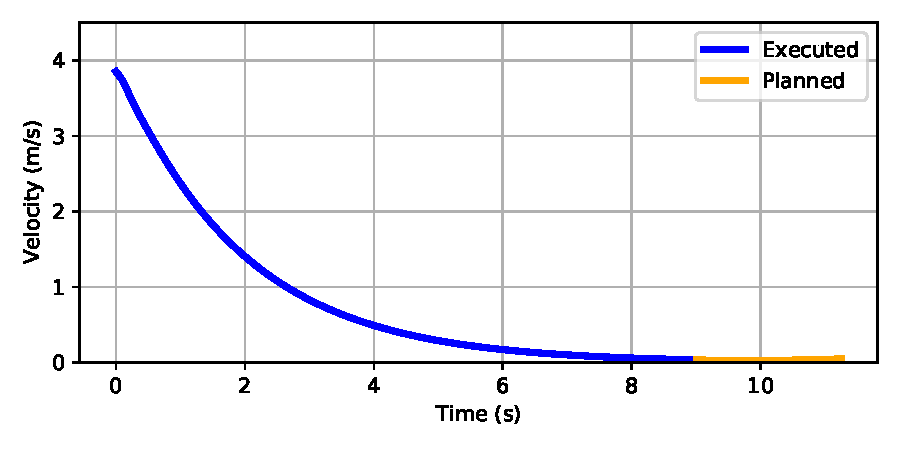
\includegraphics[width=0.8\linewidth]{figures/stop_sign_velocity.pdf}
 	\vspace{-1em}
 	\caption{Velocity in stop sign test vs time. The desired speed was 4 m/s.} 	 	\label{fig:stop_sign_velocity}
 \end{figure}
 
  \subsection{Following another vehicle}
 
 %\begin{figure}[h!]
 % 	\centering
 % 	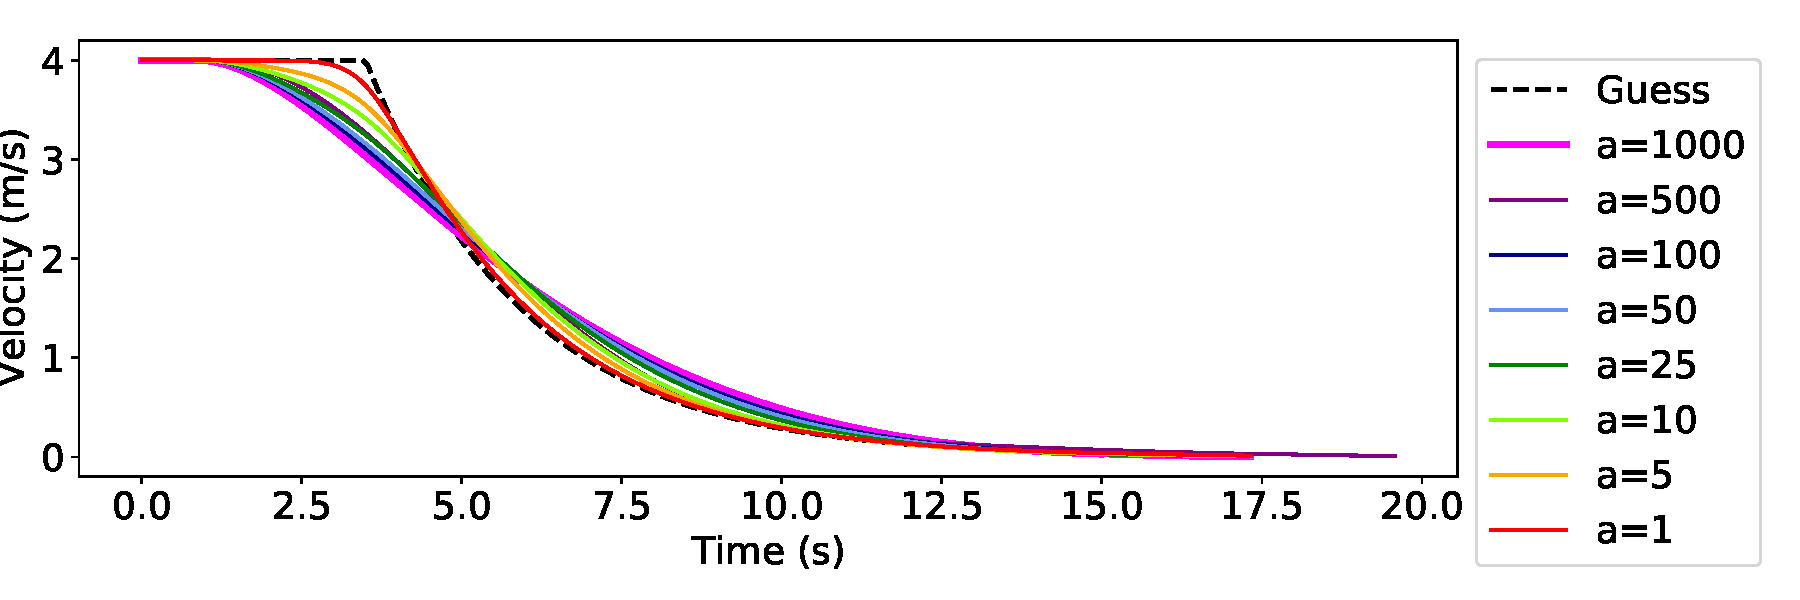
\includegraphics[width=1.0\linewidth]{figures/Velocity_time(stop).pdf}
 % 	\\
 % 	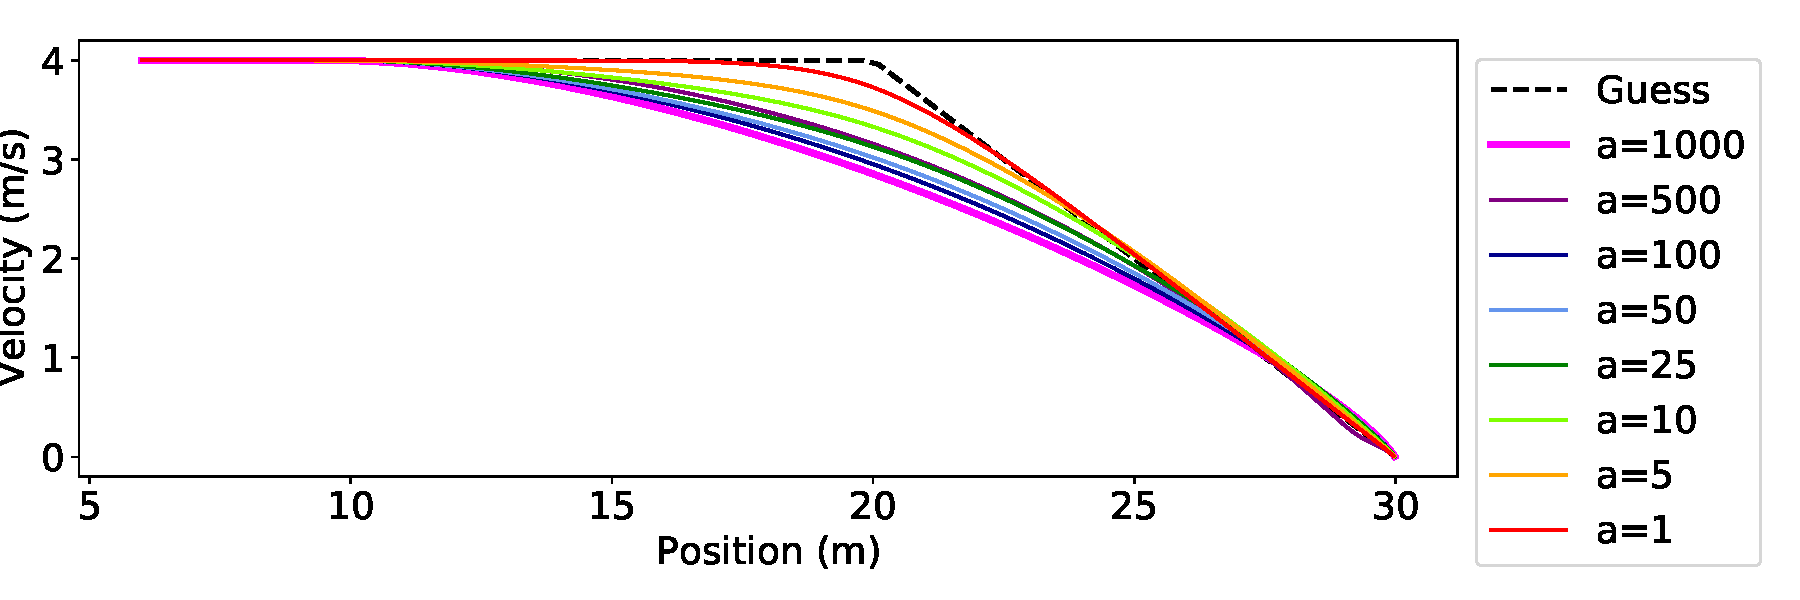
\includegraphics[width=1.0\linewidth]{figures/Velocity_position(stop).pdf}
 % 	\caption{Velocity vs time (top) and position(bottom) for the stop sign scenario. The desired or estimated velocity decreases linearly with position.}
 % 	\label{fig:velocity(stop)}
 % \end{figure}
 
 \begin{figure}[h!]
 	\centering
 	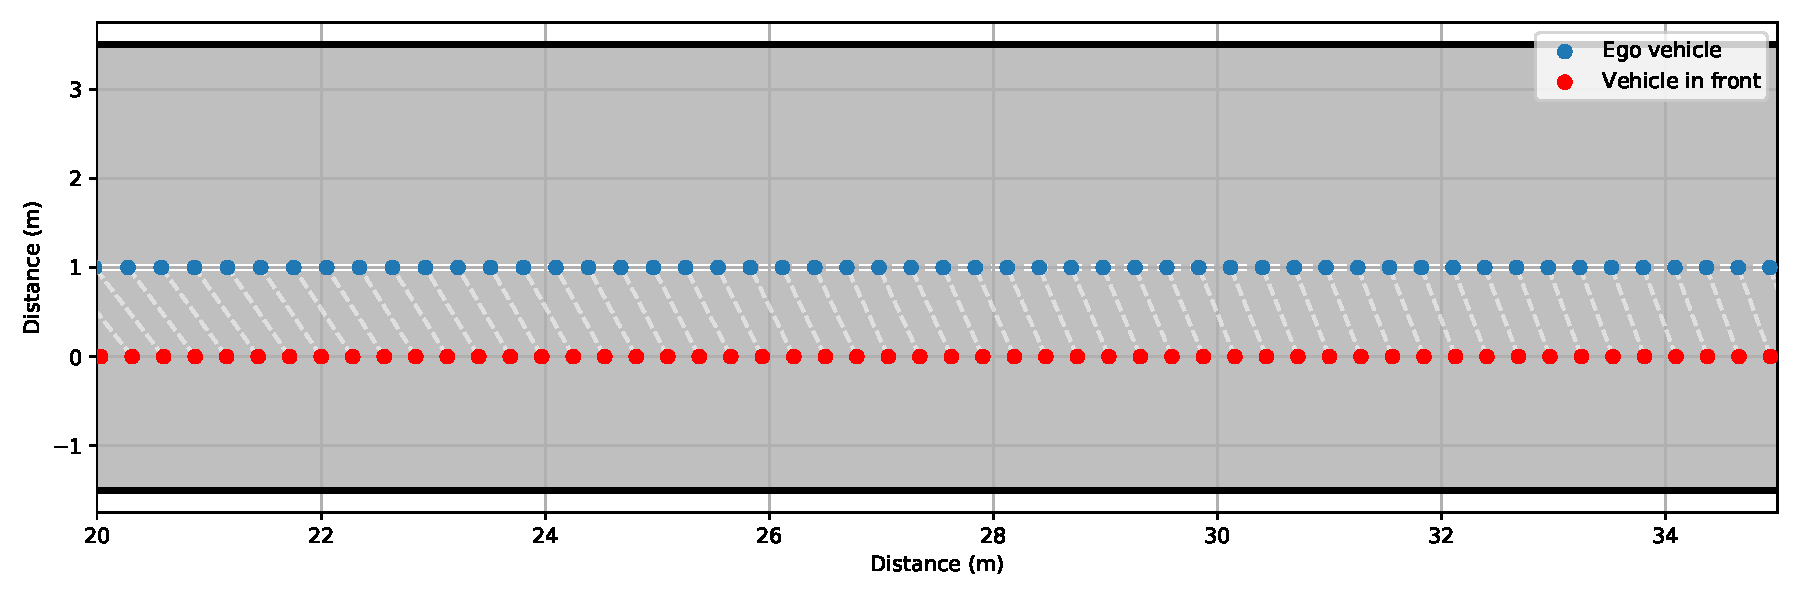
\includegraphics[width=1.0\linewidth]{figures/vehicle_following.pdf}
 	 	\vspace{-1.5em}
 	\caption{Following a slower car. The desired speed is 4 m/s but the car ahead is traveling at 3.75 m/s. The white lines connect the two vehicle's positions at each time step, showing how a safe distance is maintained.}
        \label{fig:vehicle_following}
 \end{figure}
 
The hard constraint causes the vehicle's speed to decrease, maintaining a safe distance from a slower car. Fig. \ref{fig:vehicle_following} shows the position of each vehicle over time.
 
 \begin{figure}[h!]
	\centering
	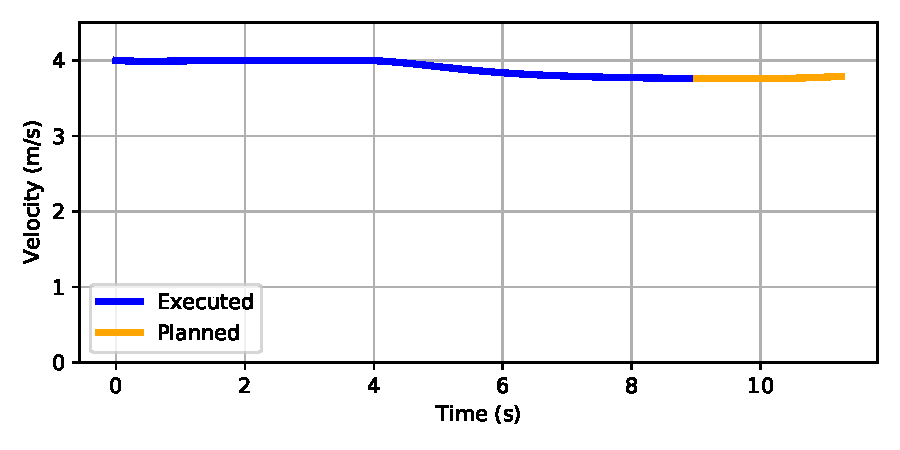
\includegraphics[width=0.8\linewidth]{figures/vehicle_following_velocity.pdf}
	 	\vspace{-1em}
	\caption{Ego vehicle velocity decreases to maintain a safe distance from another car.}		\label{fig:vehicle_following_velocity}
\end{figure}

 %Finally, to select one set of weights for \eqref{eq:costfinal} we measured both the maximum jerk and the total jerk (computed by numerical integration). Table \ref{tab:jerk(stop)} summarizes these results. The result with $a=25$, corresponding to a cost function of
 %$$J = \Big( J_{\text{accuracy}} + 10^3J_{\text{speed}} \Big) + 25\Big( 10J_\text{{jerk}} + 10J_\text{{accel}} + J_{\text{steering}}\Big),$$
 %resulted in both low total jerk (0.00177 $\text{m}/\text{s}^2$) and low maximum jerk (0.3085 $\text{m}/\text{s}^3$) so it it may be a good candidate for future tests.
% 
% \begin{table}[h]
% 	\centering
% 	\renewcommand{\arraystretch}{1.25}
% 	\begin{tabular}{|l|cc|}
% 		\hline
% 		$a$ & Total jerk ($\text{m}/\text{s}^2$) & Maximum jerk ($\text{m}/\text{s}^3$)
% 		\\\hline
% 		$a=1000$ & 0.00063 & 0.5048
% 		\\
% 		$a=500$ & 0.00976 & 0.2562\\
% 		$a=100$ & 0.00325 & 0.36873\\
% 		$a=50$ & 0.00285 & 0.3468\\
% 		$a=25$ & 0.00177 & 0.3085\\
% 		$a=10$ & 0.00526 & 0.3618\\
% 		$a=5$ & 0.00693 & 0.5699\\
% 		$a=1$ & 0.00807 & 1.2094\\\hline
% 	\end{tabular}
% 	\vspace{0.5em}
% 	\caption{Jerk applied during stopping maneuver for different MPC cost weights.}
% 	\label{tab:jerk(stop)}
% \end{table}
% 
% \subsection{Changing parameters}
% Using an optimizing algorithm enables software reusability by allowing the same MPC software to be swapped between vehicles with different parameters. To demonstrate changing the vehicle parameters with the simple kinematic model \eqref{eq:kinematic} we will move the vehicle CG forward and backward, a situation that could occur as passengers and cargo are loaded and unloaded.
% 
% %\begin{figure}[h]
%% 	\centering
%% 	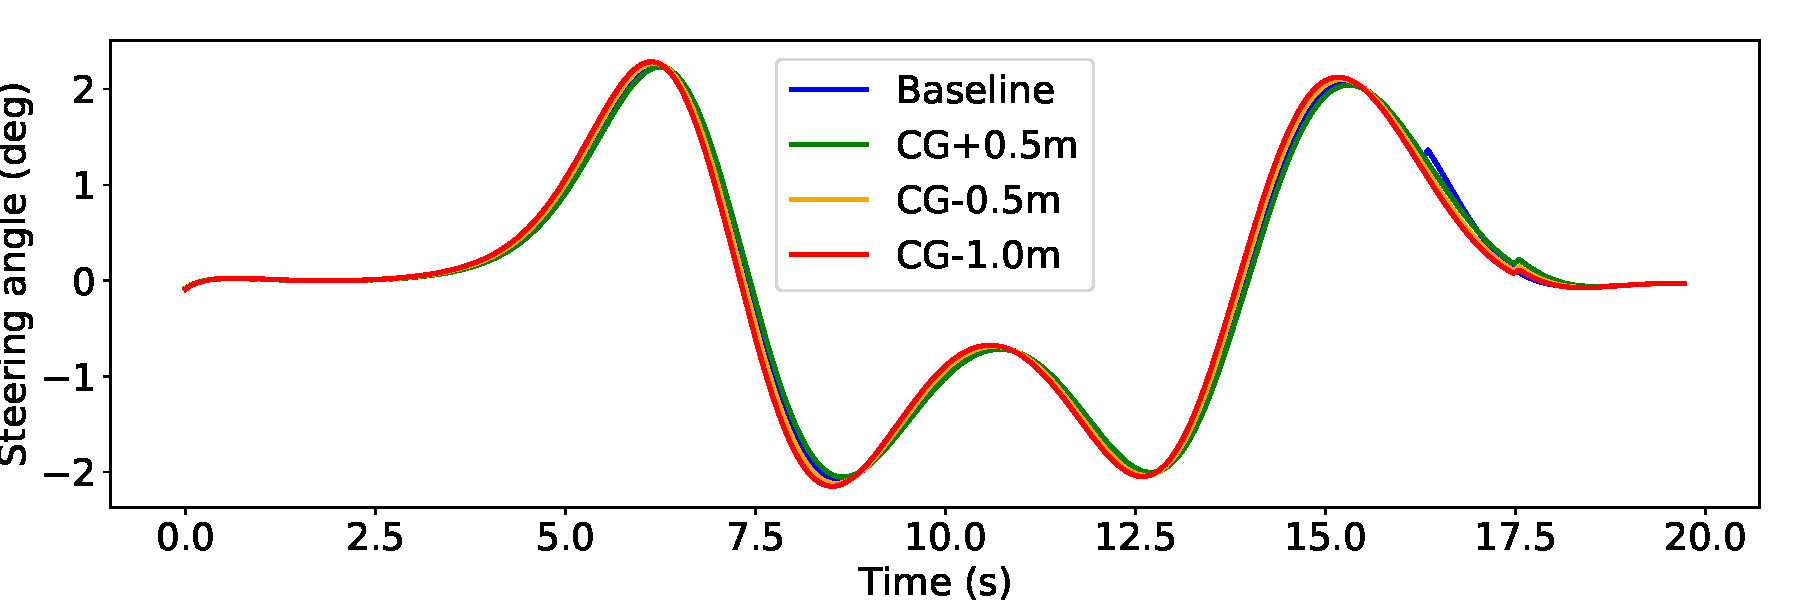
\includegraphics[width=1.0\linewidth]{figures/Steering(param).pdf}
%% 	\\
%% 	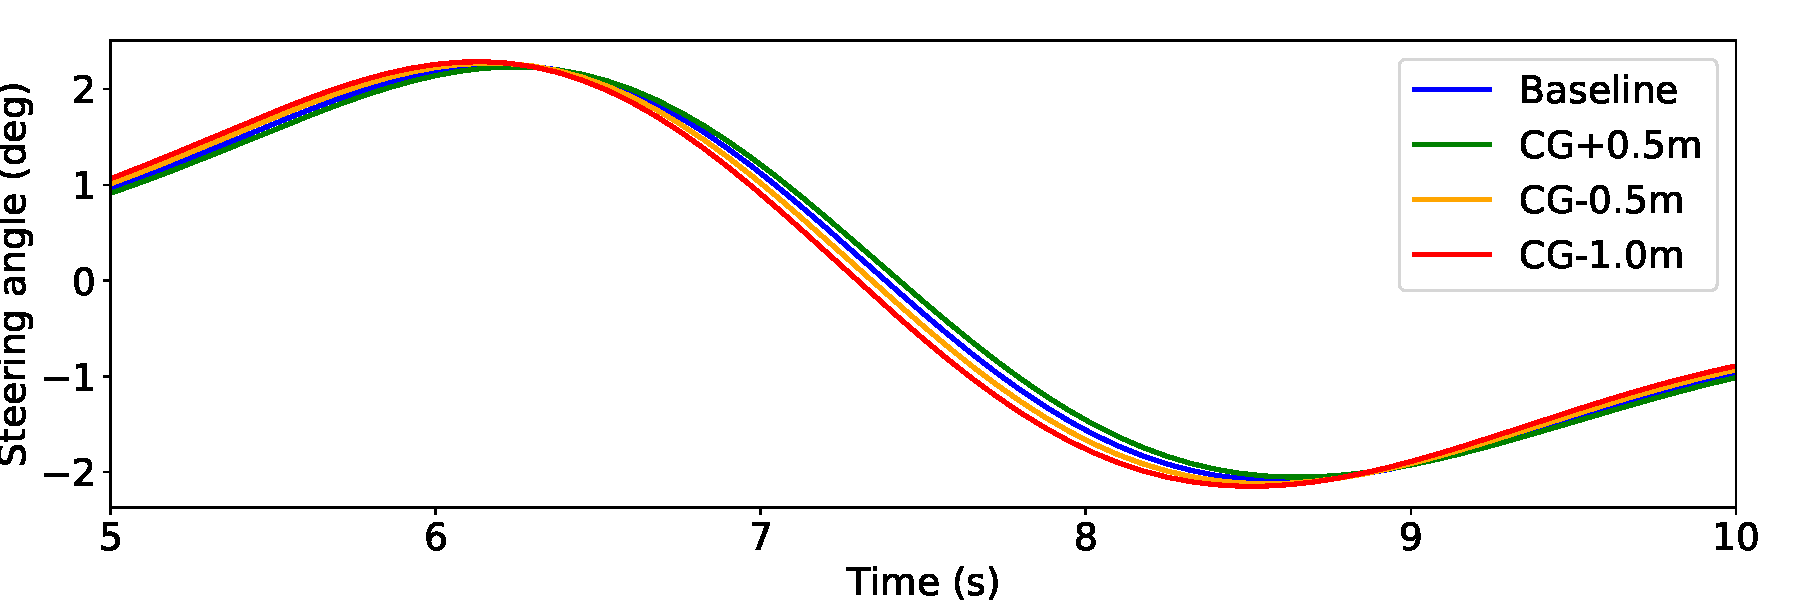
\includegraphics[width=1.0\linewidth]{figures/Steering_closeup(param).pdf}
%% 	\caption{Steering control signal for varying vehicle CG in the double-lane-change scenario (top). A close-up inspection (bottom) shows the controller begins steering earlier when the CG changes. This makes sense since the change makes the vehicle less maneuverable.}
%% 	\label{fig:Steering(param)}
%% \end{figure}
% 
%Despite the changed dynamics, the resulting position error on the double lane-change scenario (Fig. \ref{fig:position(param)}) is almost identical to the baseline. The controller produces consistent results despite parameter changes.
% 
%% \begin{figure}[h!]
%% 	\centering
%% 	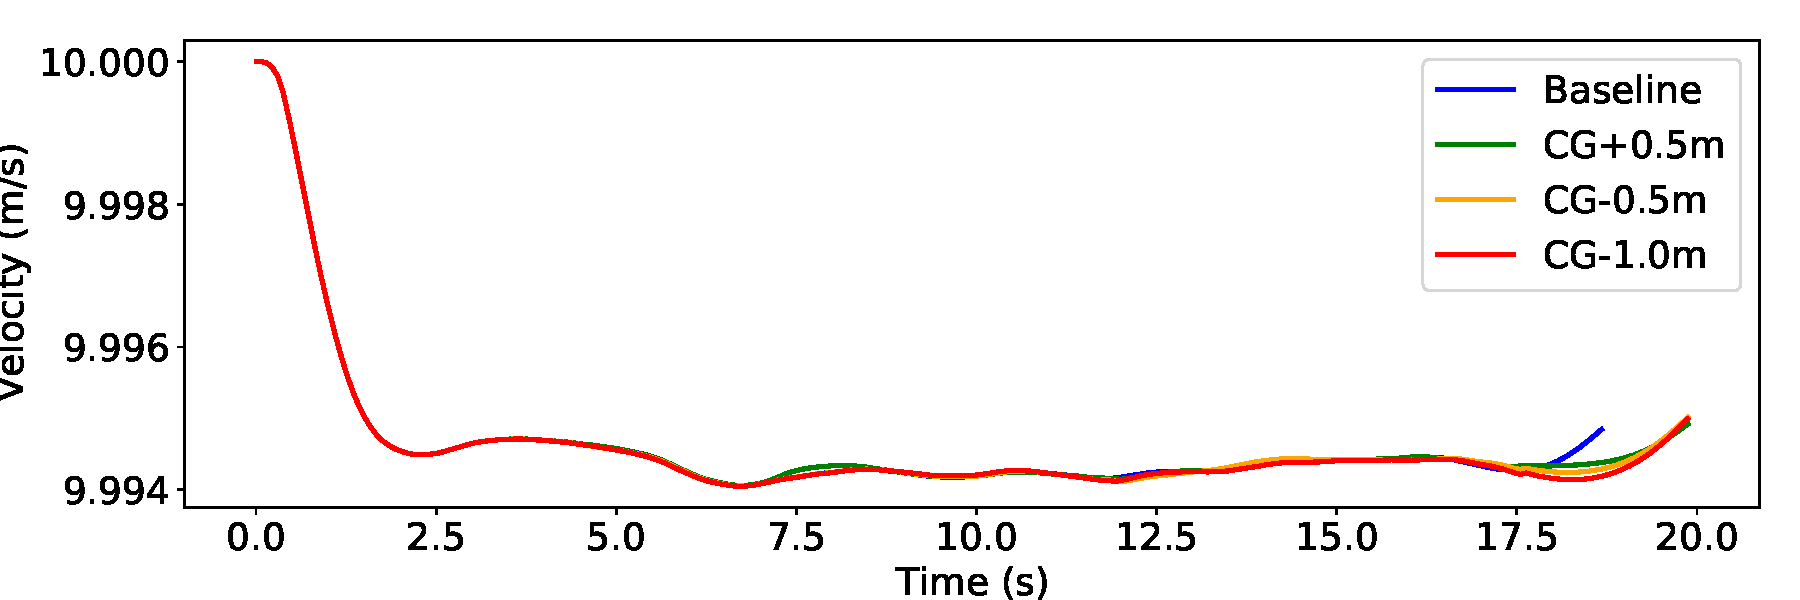
\includegraphics[width=1.0\linewidth]{figures/Velocity(param).pdf}
%% 	\caption{Velocity is almost unchanged despite changing the model parameters.}
%% 	\label{fig:velocity(param)}
%% \end{figure}
% 
% \begin{figure}[h!]
% 	\centering
% 	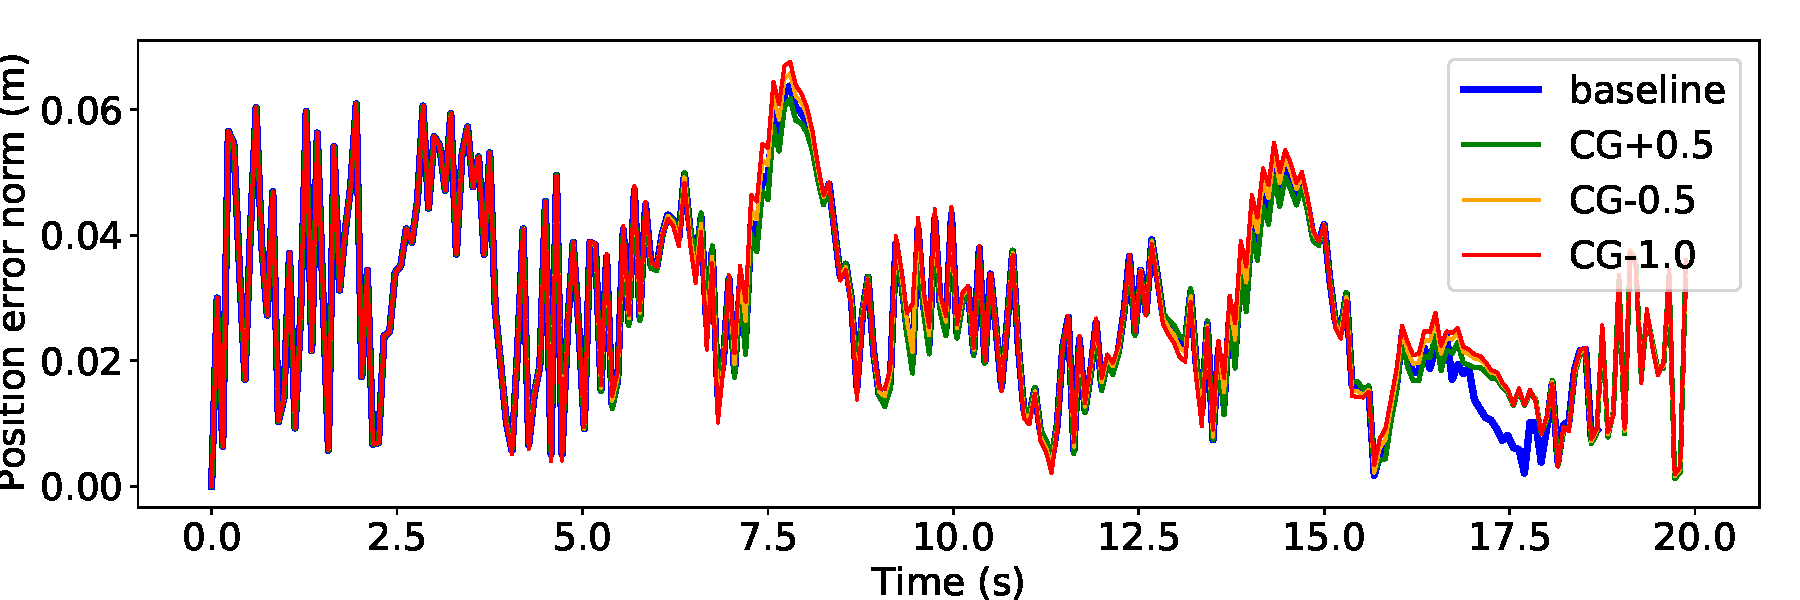
\includegraphics[width=1.0\linewidth]{figures/Position_error(param).pdf}
% 	\caption{Position error is unchanged despite changing the model parameters.}
% 	\label{fig:position(param)}
% \end{figure}
% 
   
\section{CONCLUSIONS}

In this paper we defined an API for the trajectory planning module of an autonomous driving stack (Fig. \ref{fig:block}). The inputs to this module consist of information about the driveable corridor, constraints imposed by obstacles and rules of the road, and a desired speed: all information that can be provided by higher-level software with little knowledge of vehicle hardware. Therefore, the higher-level software can be certified once and installed on different AV platforms.
We also demonstrate an NMPC trajectory planner that implements this API. The trajectory planner contains hardware-specific parameters, but can be ported to similar vehicles by changing said parameters. The controller is of similar design to other recent work \cite{nmpc_micheli}, suggesting the relevance of this software reusability-focused design to current research in NMPC AV controllers.

%A conclusion section is not required. Although a conclusion may review the main points of the paper, do not replicate the abstract as the conclusion. A conclusion might elaborate on the importance of the work or suggest applications and extensions. 

\addtolength{\textheight}{-12cm}   % This command serves to balance the column lengths
                                  % on the last page of the document manually. It shortens
                                  % the textheight of the last page by a suitable amount.
                                  % This command does not take effect until the next page
                                  % so it should come on the page before the last. Make
                                  % sure that you do not shorten the textheight too much.

%%%%%%%%%%%%%%%%%%%%%%%%%%%%%%%%%%%%%%%%%%%%%%%%%%%%%%%%%%%%%%%%%%%%%%%%%%%%%%%%



%%%%%%%%%%%%%%%%%%%%%%%%%%%%%%%%%%%%%%%%%%%%%%%%%%%%%%%%%%%%%%%%%%%%%%%%%%%%%%%%



%%%%%%%%%%%%%%%%%%%%%%%%%%%%%%%%%%%%%%%%%%%%%%%%%%%%%%%%%%%%%%%%%%%%%%%%%%%%%%%%
%\section*{APPENDIX}

%Appendixes should appear before the acknowledgment.

\section*{ACKNOWLEDGMENT}


This work was completed under Professor Sanjay Lall in the Information Systems Lab. The NMPC code was based on several open-source files provided with CasADi.
Code for this paper is published at \texttt{https://github.com/elsoroka/AutonomousCarMPC/
	tree/master/code\_for\_paper}

%%%%%%%%%%%%%%%%%%%%%%%%%%%%%%%%%%%%%%%%%%%%%%%%%%%%%%%%%%%%%%%%%%%%%%%%%%%%%%%%

%References are important to the reader; therefore, each citation must be complete and correct. If at all possible, references should be commonly available publications.


\bibliographystyle{unsrt}
\bibliography{bibliography}

\end{document}
